\section{Operationalization in the application and AI agent}
\label{sec:system}

\subsection{Scope and method-to-implementation correspondence}

This section describes the inspected version-2 implementation of the Research Map, rather than an observed pattern of use. The application turns the method's planning relations into an editable, versioned workflow. Its AI agent proposes text and comments on coherence; it does not decide whether a research design is scientifically adequate. Table~\ref{tab:method-system} separates method components present in the inspected code from partial translations and prospective capabilities. The terms in the table describe implementation, not an assessment of the method's effectiveness.

\begin{table}[htbp]
\centering
\small
\caption{Selected correspondences between the Research Map and the inspected application. ``Present'' denotes source-code behavior at the examined layer; it does not imply methodological validity or successful use in a study.}
\label{tab:method-system}
\begin{tabular}{>{\raggedright\arraybackslash}p{0.27\linewidth} >{\raggedright\arraybackslash}p{0.34\linewidth} >{\raggedright\arraybackslash}p{0.29\linewidth}}
\hline
Method component & Application representation & Boundary \\
\hline
Problem and objectives & Candidate problems, author selection, one general objective, and specific objectives & Wording and cardinality checks are proxies for conceptual fit \\
Literature and development topics & Topic units with declared objective coverage & Coverage is recorded, not independently established \\
Objective--method matrix & Per-objective collection, analysis, and expected-result fields & A general-objective synthesis row extends the original map \\
Dependency and revision & Trace links, source revisions, drafts, proposals, and stale statuses & Staleness propagates by element type, not exact graph descendant \\
Coherence and human validation & Stage checks, AI suggestions, author confirmation, and conditional advisor review & Advisor approval and advisory coherence inspection are distinct \\
\hline
\end{tabular}
\end{table}

The original map numbers five stages and places the matrix beside them \cite{franca2026map}. The software adds workflow states, reference records, a provisional title, and a synthesis row to make those relations editable and exportable. These additions are implementation decisions, not newly discovered stages of the method. Conversely, the detailed specification treats research questions as an item for validation, while the current schema stores a question in each problem candidate and a selected central problem but has no dedicated research-questions unit \cite{franca2026detail}.

\subsection{Information model and guided proposals}

The author can begin with free text or a guided intake. A server-side generative component interprets that input and returns six alternative research problems; the author selects one for further development. A Research Starter call supplies candidate bibliographic records during discovery. Subsequent routes propose or regenerate a problem statement, general and specific objectives, literature and development topics, and the objective--method matrix. Generated content is therefore a proposal within a structured authoring process, not a completed research plan or a verified literature synthesis.

The data model distinguishes \emph{proposed content} from \emph{approved content} for an element and records its type, status, revision, source revision, update actor, and associated reference identifiers. Topic units also carry declared objective coverage; matrix rows carry planned data collection, analysis or treatment, and an \emph{expected} result for each objective. Trace links record directed relations between elements. These fields make an intended connection inspectable, but a stored link does not show that the connected claims are substantively sound. Retrieved references retain provider and identifier metadata; a DOI or a provider record identifies a source, not the evidence that it supports a particular sentence.

Figure~\ref{fig:system-flowchart} follows the proposed content from researcher input through the Research Map scaffold, agent assistance, stage submission, and the role-dependent review path. The student branch includes a saved pending review, an e-mail notification attempt, and a separate advisor decision; the advisor-as-author branch advances without that external request. A static suggestion library is present in the code. The growing knowledge base and comprehensive methodological library envisaged in the detailed specification are not evidenced here as implemented learning components \cite{franca2026detail}.

\begin{figure}[htbp]
\centering
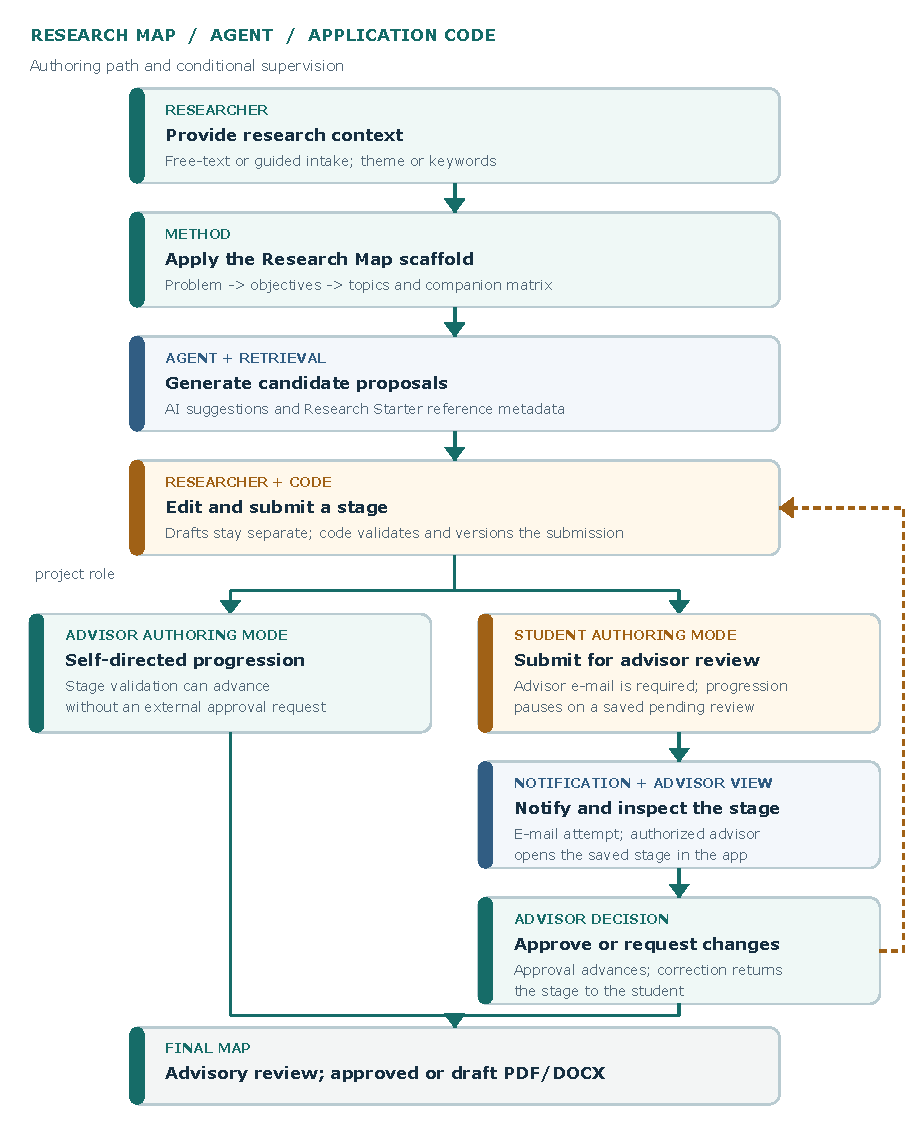
\includegraphics[width=\linewidth]{figures/system-supervision-flowchart.pdf}
\caption{Interpretive flowchart of the Research Map, agent, application code, and conditional student--advisor path in the inspected version-2 workflow. The dashed arrow denotes a request for corrections. E-mail is an attempted notification; the authenticated advisor's in-app decision controls progression. The final algorithmic coherence review remains advisory. This is not an observed user trajectory or a guarantee of scientific quality.}
\label{fig:system-flowchart}
\end{figure}

\subsection{Checks, decisions, and revision}

Validation occurs at different levels. Stage routes check required fields, allowed counts, identifiers, declared topic coverage, and selected lexical relationships. For example, alignment between a problem and an objective can be approximated from wording, while matrix completeness can be checked from filled fields. Neither check establishes that the objective answers the research problem or that a proposed collection and analysis method is appropriate. A product rule also asks for a final development topic linked to the general objective or a stated methodological exception; the latter qualification matters because the source document presents the relation as guidance, not a universal constraint \cite{franca2026detail}.

Drafts and AI proposals are stored separately from the currently confirmed unit, with the source revision from which they were produced. Saving a draft or generating a proposal does not itself replace approved academic content. A confirmation action can update the canonical unit; stale proposals based on an older context require review. Saves use revision matching to avoid silently overwriting a newer version, and changed units have recoverable history.

When confirmed academic content changes, the workflow compares content fingerprints and marks later \emph{types} of elements stale. Earlier text and historical approval remain available for inspection. A change to a literature or development topic can also mark methodology rows stale. This propagation is intentionally conservative: it follows a predefined type-dependency map, not the exact descendants of each stored trace link. The user must revisit affected content and decide what to retain, revise, or confirm.

\subsection{Student and advisor roles}

The application distinguishes the project's \emph{authoring role} from the person who reviews a student's submission. A project authored in advisor mode follows a self-directed path: after applicable stage checks, its author can advance without an external approval request. In student mode, the project must have an advisor e-mail address before a stage can be submitted for advancement, although a draft may still be saved. Submission creates a pending review record for that stage, with its source revision and proposed next state. The stage remains awaiting review and academic confirmation or forward progression is restricted while that request is pending. This applies to submitted units such as the problem, objectives, topic groups, methodology matrix, and final map; it does not mean that every keystroke or initial prompt is individually approved.

After a pending review is saved, the server attempts to notify the registered advisor by e-mail. The message identifies the project and stage and links back to the application. The notification requires a configured mail provider and a usable recipient address; a skipped or failed send does not itself cancel the saved review request. Thus the implementation supports e-mail notification but cannot, from the request path alone, establish delivery to the advisor's inbox or that the message was read. The advisor's review authority comes from authenticated project access in the application, not from possession of the e-mail link.

In the advisor workspace, the reviewer can inspect the submitted stage in the context of the student's map and save a comment, approve it, or request changes. A request for changes requires a comment and returns the stage for student revision and resubmission. Approval records the advisor's decision and applies the pending transition, allowing the student to continue; for the final map, this can establish the current final approval used by the export path. The application also attempts to notify the student of the advisor's comment or decision. This human approval is a product workflow decision and is distinct from the final algorithmic coherence findings described below. Neither author of this paper is represented as having reviewed a student submission for the present descriptive article.

\subsection{Final review and export}

The final map assembles nodes for the input, selected problem, objectives, topics, matrix rows, title, and associated references. Stored trace links and reference associations provide graph edges; deterministic checks can detect orphan edges, cycles, absent elements, and other structural findings. A model-assisted coherence pass adds suggestions or a warning if that pass is unavailable. These findings support inspection. They are not a proof of semantic coherence, feasibility, or likely research outcomes.

The distinction between a check and a completion gate is material. The current completion route invokes the final-map predicate in \emph{advisory} mode, which permits completion despite findings that strict mode would classify as blocking. It then excludes blocking findings from the persisted final summary while retaining non-blocking revision guidance. Earlier stage validation can still reject malformed or incomplete inputs. Accordingly, the present implementation should be described as offering a final traceability and coherence review, not enforcing a guarantee that the completed plan is internally consistent.

For the version-2 workflow, export requires a completed or reviewing map and either current final approval or an explicitly requested draft. PDF and DOCX are rendered from a shared report model without another AI generation call. They contain the proposed research plan, its planned methods and expected results, associated references, and available review warnings. The exported document is a planning artifact; its expected results are not findings from a study. The next section uses a constructed case to make the authoring and revision path concrete without presenting it as user-study evidence.
